\section{Zustands-Regler}
\subsection{State Feadback}

$A_g = A-BK \; , \; B_g = BK_{vf} \; , \; C_g = C $\\
$G(s) = \frac{\underline{Y}(s)}{\underline{U}(s)} = C(sI-A+BK)^{-1}BK_{vf}$\\
$K_{vf} = (C(-A+BK)^{-1}B)^{-1}$

\subsection{Pole Placement}

\begin{tabular}{ll}
	\parbox{8cm}{$det(\lambda I-A+BK) = (\lambda - \lambda_1)...(\lambda - \lambda_n)$} &
	\parbox{3cm}{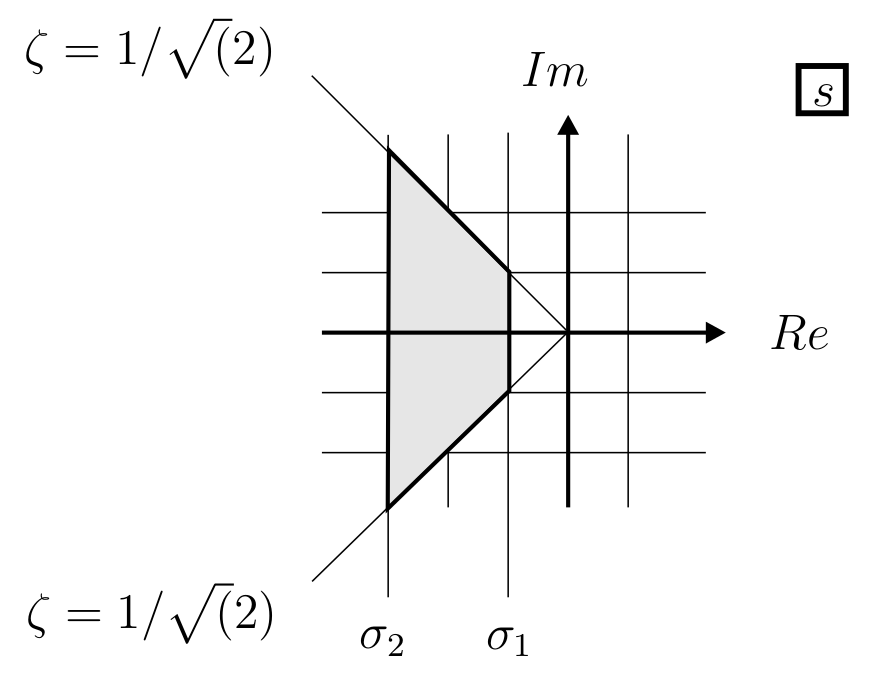
\includegraphics[width=3cm]{./bilder/pole_locations.png}}
\end{tabular}

\newpage

\subsection{LQR-Entwurf (Linear-quadratic regulator)}
	\begin{tabular}{ll}
		\parbox{6cm}{	$J(K_R,T_N,\ldots)=\int\limits^{\infty}_0 e(t)^2 dt = minimal$\\
						$J=\int\limits_0^{\infty} {x^T Q x+u^T R u}= minimal$\\}&
		\parbox{6cm}{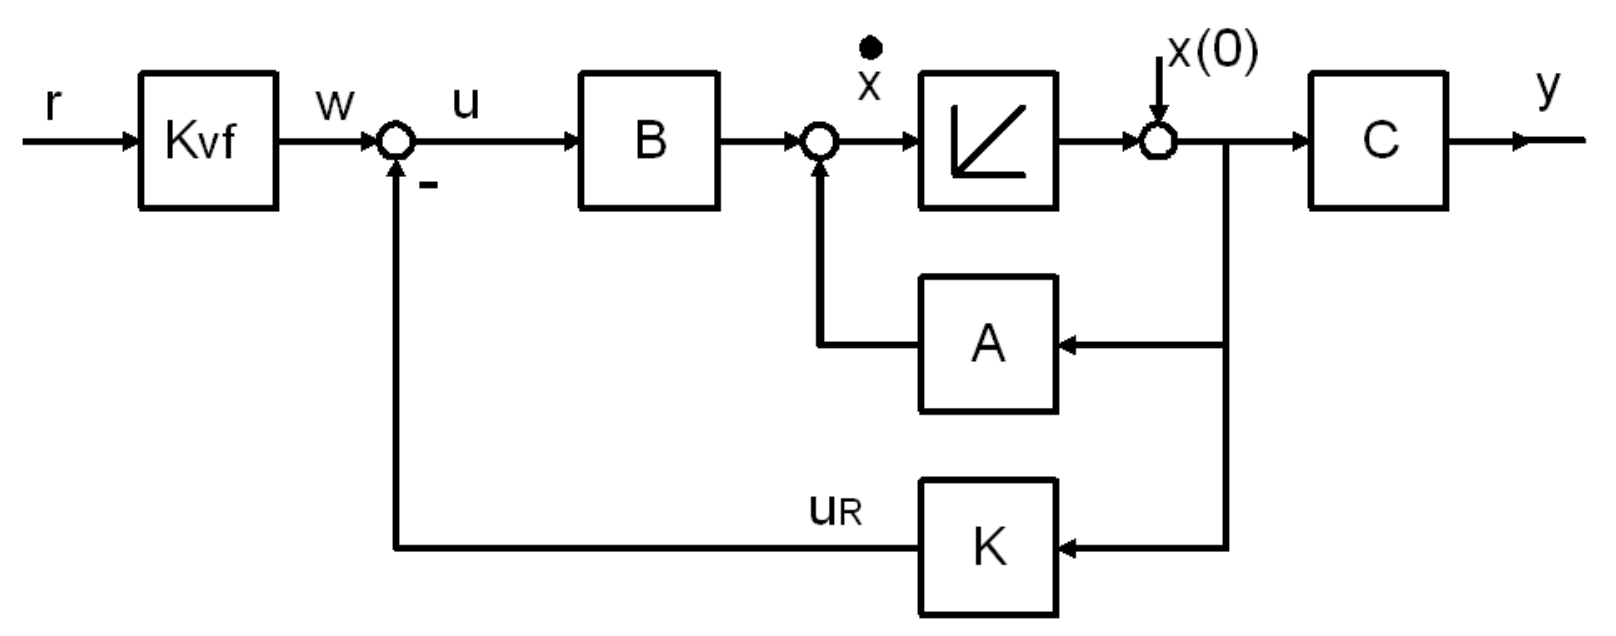
\includegraphics[width=6cm]{./bilder/statereg.png}}
	\end{tabular}\\	
	Q,R: positive definite; Bei SISO ist R eine Zahl\\
	Optimum: Riccati equation\\
	$ A^T P + P A - P B R^{-1} B^T P = -Q$ \hspace{2cm}
	P ist die L"osungsmatrix
	\begin{aufzaehlung}
    	\item $\dot{x} = Ax + Bu \; / \;  Q \; \text{und} \; R \; \text{gegeben}$
    	\textbf{meist} wird f"ur Q=I und R=1 eingesetzt.
    	\item L"osungsmatrix P bestimmen (aus der L"osungsmenge den positiv
    	definierten Wert)
    	\item Reglervektor berechnen $K=R^{-1} B^T P$
    \end{aufzaehlung}

\subsection{LQG-Entwurf (Linear-quadratic gaussian / Observer)}
	\begin{tabular}{ll}
		\parbox{12cm}{	Duale Korrespondenzen:\\
						\begin{eqnarray*}
						\textbf{LQR} &\Leftrightarrow& \textbf{LQG} \\
						P_c &\Leftrightarrow& P_o^T\\
						B &\Leftrightarrow& C^T\\
						A &\Leftrightarrow& A^T\\
						K &\Leftrightarrow& H^T\\
						A - BK &\Leftrightarrow& A - HC\\
						det(\lambda I-A+BK) &\Leftrightarrow& det(\lambda I-A+HC) \\
						A^T P + P A - P B R^{-1} B^T P = -Q &\Leftrightarrow& A P + P A^T - P C^T R^{-1} C P = -Q \\
						K=R^{-1} B^T P &\Leftrightarrow& H=(R^{-1} CP)^T = PC^TR^{-1}
						\end{eqnarray*}
					}
		\parbox{6cm}{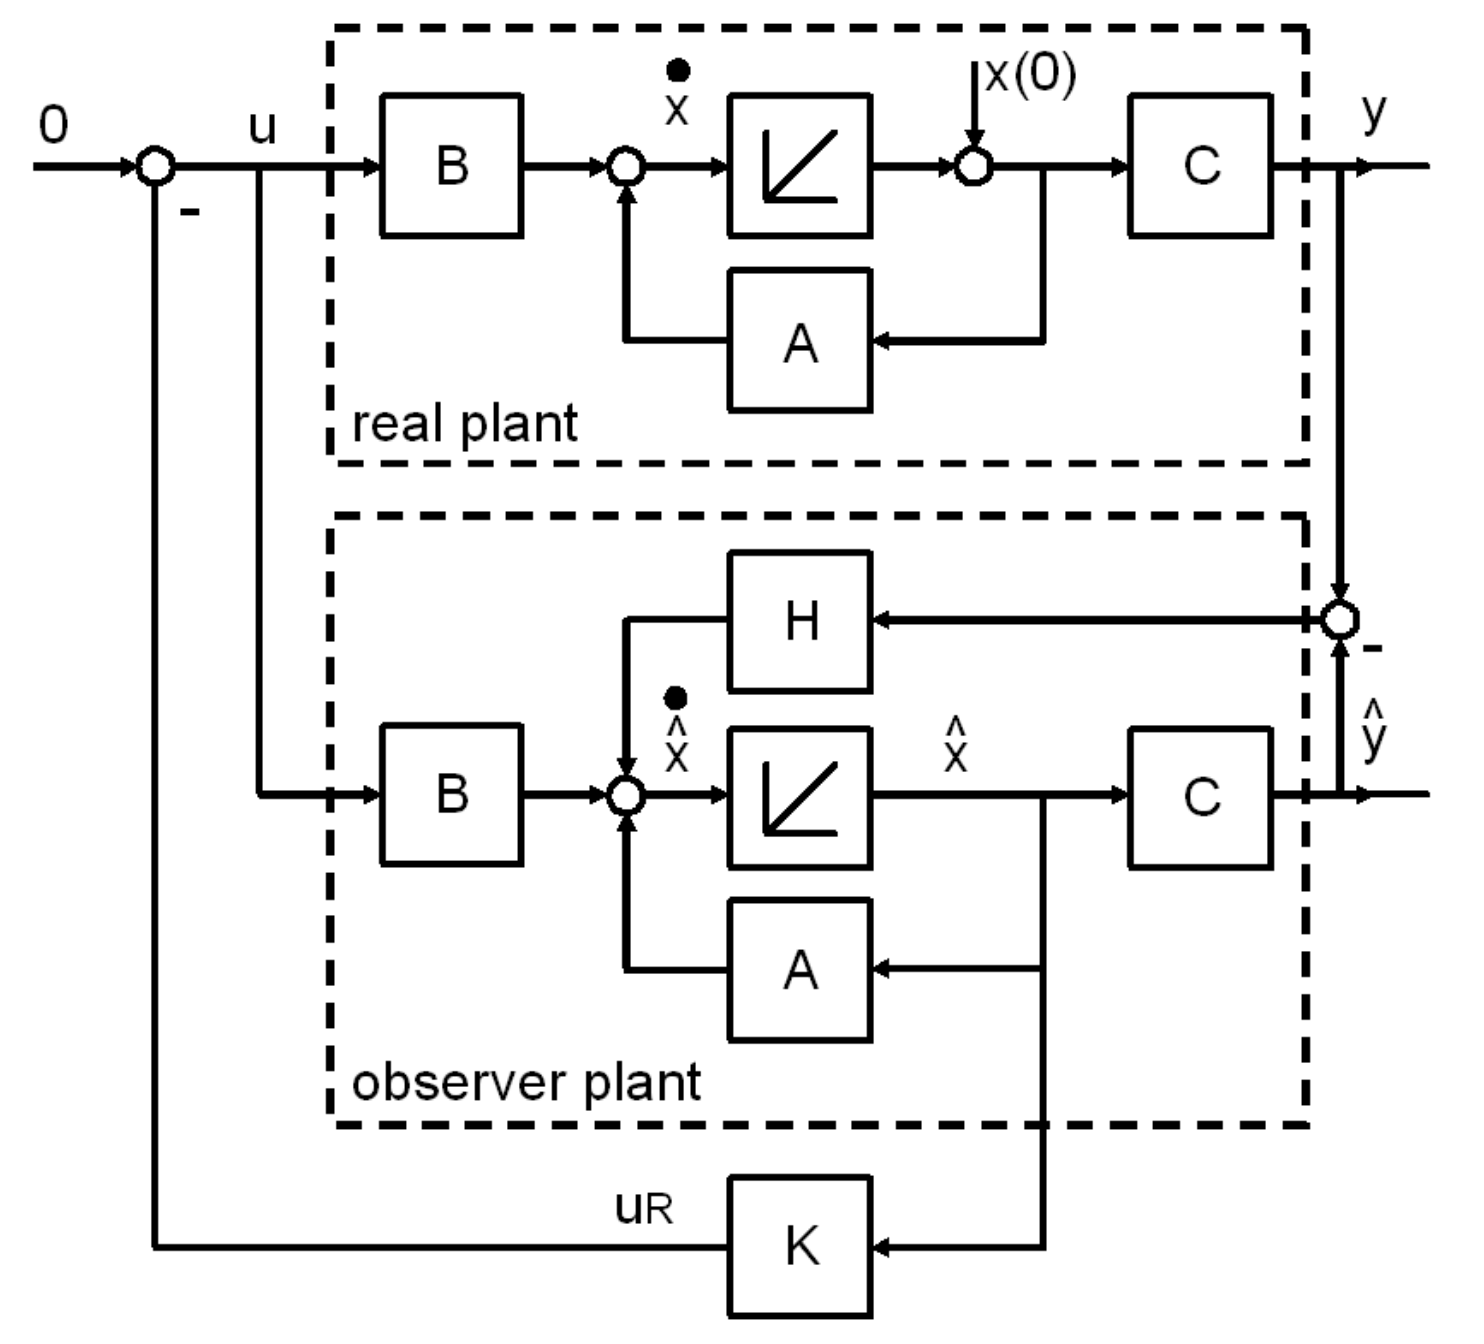
\includegraphics[width=6cm]{./bilder/observer.png}}
	\end{tabular}\\
	
\subsection{LQR/LQG Entwurf}
\begin{tabular}{ll}
	\parbox{6cm}{Gesamtsystem: \\ $
			\begin{bmatrix}
				\dot{x}\\
				\dot{\tilde{x}}\\
			\end{bmatrix} = 
			\begin{bmatrix}
				A-BK && BK\\
				0 && A-HC\\
			\end{bmatrix} 
			\begin{bmatrix}
				x\\
				\tilde{x}\\
			\end{bmatrix}
			$} &
	\parbox{6cm}{Charakteristik:\\ $
			det 
			\begin{bmatrix}
				sI - A + BK && -BK\\
				0 && sI - A + HC\\
			\end{bmatrix}=$\\
			$det(sI-A+BK)*det(sI-A+HC)=0$}
\end{tabular}
	
\subsection{LQR/LTR und LQR/LTR Entwurf}

\begin{tabular}{ll}
	\parbox{8cm}{
		LQR/LTR
		\begin{itemize}
			\item LQR beliebige Gewichtung
			\item LQG mit $Q=\rho BB^T \; / \; R=I  \; / \; \rho > 0$
		\end{itemize}}
	\parbox{8cm}{
			LQG/LTR
			\begin{itemize}
				\item LQR mit $Q=\rho C^TC \; / \; R=I  \; / \; \rho > 0$
				\item LQG beliebige Gewichtung
			\end{itemize}}
\end{tabular}		
